% Options for packages loaded elsewhere
\PassOptionsToPackage{unicode}{hyperref}
\PassOptionsToPackage{hyphens}{url}
\PassOptionsToPackage{dvipsnames,svgnames,x11names}{xcolor}
%
\documentclass[
  article,
  nofooter]{jss}

\usepackage{amsmath,amssymb}
\usepackage{iftex}
\ifPDFTeX
  \usepackage[T1]{fontenc}
  \usepackage[utf8]{inputenc}
  \usepackage{textcomp} % provide euro and other symbols
\else % if luatex or xetex
  \usepackage{unicode-math}
  \defaultfontfeatures{Scale=MatchLowercase}
  \defaultfontfeatures[\rmfamily]{Ligatures=TeX,Scale=1}
\fi
\usepackage{lmodern}
\ifPDFTeX\else  
    % xetex/luatex font selection
\fi
% Use upquote if available, for straight quotes in verbatim environments
\IfFileExists{upquote.sty}{\usepackage{upquote}}{}
\IfFileExists{microtype.sty}{% use microtype if available
  \usepackage[]{microtype}
  \UseMicrotypeSet[protrusion]{basicmath} % disable protrusion for tt fonts
}{}
\makeatletter
\@ifundefined{KOMAClassName}{% if non-KOMA class
  \IfFileExists{parskip.sty}{%
    \usepackage{parskip}
  }{% else
    \setlength{\parindent}{0pt}
    \setlength{\parskip}{6pt plus 2pt minus 1pt}}
}{% if KOMA class
  \KOMAoptions{parskip=half}}
\makeatother
\usepackage{xcolor}
\setlength{\emergencystretch}{3em} % prevent overfull lines
\setcounter{secnumdepth}{-\maxdimen} % remove section numbering
% Make \paragraph and \subparagraph free-standing
\ifx\paragraph\undefined\else
  \let\oldparagraph\paragraph
  \renewcommand{\paragraph}[1]{\oldparagraph{#1}\mbox{}}
\fi
\ifx\subparagraph\undefined\else
  \let\oldsubparagraph\subparagraph
  \renewcommand{\subparagraph}[1]{\oldsubparagraph{#1}\mbox{}}
\fi


\providecommand{\tightlist}{%
  \setlength{\itemsep}{0pt}\setlength{\parskip}{0pt}}\usepackage{longtable,booktabs,array}
\usepackage{calc} % for calculating minipage widths
% Correct order of tables after \paragraph or \subparagraph
\usepackage{etoolbox}
\makeatletter
\patchcmd\longtable{\par}{\if@noskipsec\mbox{}\fi\par}{}{}
\makeatother
% Allow footnotes in longtable head/foot
\IfFileExists{footnotehyper.sty}{\usepackage{footnotehyper}}{\usepackage{footnote}}
\makesavenoteenv{longtable}
\usepackage{graphicx}
\makeatletter
\def\maxwidth{\ifdim\Gin@nat@width>\linewidth\linewidth\else\Gin@nat@width\fi}
\def\maxheight{\ifdim\Gin@nat@height>\textheight\textheight\else\Gin@nat@height\fi}
\makeatother
% Scale images if necessary, so that they will not overflow the page
% margins by default, and it is still possible to overwrite the defaults
% using explicit options in \includegraphics[width, height, ...]{}
\setkeys{Gin}{width=\maxwidth,height=\maxheight,keepaspectratio}
% Set default figure placement to htbp
\makeatletter
\def\fps@figure{htbp}
\makeatother
% definitions for citeproc citations
\NewDocumentCommand\citeproctext{}{}
\NewDocumentCommand\citeproc{mm}{%
  \begingroup\def\citeproctext{#2}\cite{#1}\endgroup}
\makeatletter
 % allow citations to break across lines
 \let\@cite@ofmt\@firstofone
 % avoid brackets around text for \cite:
 \def\@biblabel#1{}
 \def\@cite#1#2{{#1\if@tempswa , #2\fi}}
\makeatother
\newlength{\cslhangindent}
\setlength{\cslhangindent}{1.5em}
\newlength{\csllabelwidth}
\setlength{\csllabelwidth}{3em}
\newenvironment{CSLReferences}[2] % #1 hanging-indent, #2 entry-spacing
 {\begin{list}{}{%
  \setlength{\itemindent}{0pt}
  \setlength{\leftmargin}{0pt}
  \setlength{\parsep}{0pt}
  % turn on hanging indent if param 1 is 1
  \ifodd #1
   \setlength{\leftmargin}{\cslhangindent}
   \setlength{\itemindent}{-1\cslhangindent}
  \fi
  % set entry spacing
  \setlength{\itemsep}{#2\baselineskip}}}
 {\end{list}}
\usepackage{calc}
\newcommand{\CSLBlock}[1]{\hfill\break\parbox[t]{\linewidth}{\strut\ignorespaces#1\strut}}
\newcommand{\CSLLeftMargin}[1]{\parbox[t]{\csllabelwidth}{\strut#1\strut}}
\newcommand{\CSLRightInline}[1]{\parbox[t]{\linewidth - \csllabelwidth}{\strut#1\strut}}
\newcommand{\CSLIndent}[1]{\hspace{\cslhangindent}#1}

\usepackage{orcidlink,thumbpdf,lmodern}

\newcommand{\class}[1]{`\code{#1}'}
\newcommand{\fct}[1]{\code{#1()}}
\makeatletter
\@ifpackageloaded{caption}{}{\usepackage{caption}}
\AtBeginDocument{%
\ifdefined\contentsname
  \renewcommand*\contentsname{Table of contents}
\else
  \newcommand\contentsname{Table of contents}
\fi
\ifdefined\listfigurename
  \renewcommand*\listfigurename{List of Figures}
\else
  \newcommand\listfigurename{List of Figures}
\fi
\ifdefined\listtablename
  \renewcommand*\listtablename{List of Tables}
\else
  \newcommand\listtablename{List of Tables}
\fi
\ifdefined\figurename
  \renewcommand*\figurename{Figure}
\else
  \newcommand\figurename{Figure}
\fi
\ifdefined\tablename
  \renewcommand*\tablename{Table}
\else
  \newcommand\tablename{Table}
\fi
}
\@ifpackageloaded{float}{}{\usepackage{float}}
\floatstyle{ruled}
\@ifundefined{c@chapter}{\newfloat{codelisting}{h}{lop}}{\newfloat{codelisting}{h}{lop}[chapter]}
\floatname{codelisting}{Listing}
\newcommand*\listoflistings{\listof{codelisting}{List of Listings}}
\makeatother
\makeatletter
\makeatother
\makeatletter
\@ifpackageloaded{caption}{}{\usepackage{caption}}
\@ifpackageloaded{subcaption}{}{\usepackage{subcaption}}
\makeatother
\makeatletter
\@ifpackageloaded{tcolorbox}{}{\usepackage[skins,breakable]{tcolorbox}}
\makeatother
\makeatletter
\@ifundefined{shadecolor}{\definecolor{shadecolor}{rgb}{.97, .97, .97}}{}
\makeatother
\makeatletter
\makeatother
\makeatletter
\ifdefined\Shaded\renewenvironment{Shaded}{\begin{tcolorbox}[frame hidden, sharp corners, breakable, boxrule=0pt, borderline west={3pt}{0pt}{shadecolor}, interior hidden, enhanced]}{\end{tcolorbox}}\fi
\makeatother
\ifLuaTeX
  \usepackage{selnolig}  % disable illegal ligatures
\fi
\usepackage{bookmark}

\IfFileExists{xurl.sty}{\usepackage{xurl}}{} % add URL line breaks if available
\urlstyle{same} % disable monospaced font for URLs
\hypersetup{
  pdftitle={Why Americans Travel: Predicting Trip Purpose from the National Household Travel Survey},
  colorlinks=true,
  linkcolor={blue},
  filecolor={Maroon},
  citecolor={Blue},
  urlcolor={Blue},
  pdfcreator={LaTeX via pandoc}}

%% -- Article metainformation (author, title, ...) -----------------------------

%% Author information
\author{Marion Bauman\\Georgetown University \And Aaron
Schwall\\Georgetown University \AND Varun Patel\\Georgetown
University \And Yuhan Cui\\Georgetown University}
\Plainauthor{Marion Bauman, Aaron Schwall, Varun Patel, Yuhan
Cui} %% comma-separated

\title{Why Americans Travel: Predicting Trip Purpose from the National
Household Travel Survey}
\Plaintitle{Why Americans Travel: Predicting Trip Purpose from the
National Household Travel Survey} %% without formatting

%% an abstract and keywords
\Abstract{In this study, we examine data from the National Highway
Travel Survey (NHTS), which is conducted yearly by the Federal Highway
Administration (FHWA) to gather information about household travel
habits (Federal Highway Administration 2022a). We examine data from the
2022 survey and train five models in an attempt to accurately predict
the trip purpose. The models trained include logistic regression,
support vector machine (SVM), nueral network, random forest, and
XGBoost. We find that XGBoost performs the best with a test accuracy
over 82 percent and a ROC AUC of 0.97. We then discuss the implications
of these results and possible future applications of these findings.}

%% at least one keyword must be supplied

%% publication information
%% NOTE: Typically, this can be left commented and will be filled out by the technical editor
%% \Volume{50}
%% \Issue{9}
%% \Month{June}
%% \Year{2012}
%% \Submitdate{2012-06-04}
%% \Acceptdate{2012-06-04}
%% \setcounter{page}{1}
%% \Pages{1--xx}

%% The address of (at least) one author should be given
%% in the following format:
\Address{
Marion Bauman\\
Department of Data Science and Statistics\\
\\~
Aaron Schwall\\
Department of Data Science and Statistics\\
\\~
Varun Patel\\
Department of Data Science and Statistics\\
\\~
Yuhan Cui\\
Department of Data Science and Statistics\\
\\~

}

\begin{document}
\maketitle

\section{Introduction}\label{introduction}

Americans are in constant transit, utilizing the national interstate and
highway system to travel various distances. Whether commuting to work,
taking vacations, visiting friends and family, transporting goods and
services, or engaging in commerce, people are constantly moving.
Understanding U.S. travel patterns provides essential insights into a
wide range of fields including environmental protection resource
allocation, urban planning, and economic trends. This research aims to
understand the motivation behind American travel based on trip
specifics. Specifically, we seek to predict the purpose of trips in
order to understand the connection between travel details and purpose
for travel.

A wide variety of industries and stakeholders are interested in
understanding travel habits and the usage of American transportation
networks, particularly after the disruption of the COVID-19 pandemic
that began in 2020. Research applications include: pedestrian studies,
bicycle studies, environmental impact, energy consumption, health,
public policty, transit planning, understanding emerging travel modes,
and identifying special population groups (Federal Highway
Administration 2023). Lu and Giuliano studied the travel habits of
different income and race groups across the pandemic, finding that lower
income and ethnic minority groups continued to travel for work and
shopping purposes. Their model using trip purpose indicated that
higher-income and White populations were able to limit travel according
to government restrictions, likely due to their higher resources and
increased ability to work from home (Lu and Giuliano 2023). Paul's
dissertation studies the vehicle-sharing its equity impacts, finding
that trip purpose is a significant predictor for whether private
vehicles are being shared (Paul 2023).

While extensive research has been conducted into the implications of
American travel habits on equity, environment, policy, and more, little
research has been done on predicting \emph{why} a person traveled based
on trip-level data, without knowing the final destination. Our research
aims to fill this gap by understanding the purpose of travel without
geospatial information. This modeling task importantly protects
individual privacy because it includes no GPS data on travel. Using
travel data such as trip length, trip timing, and demographics to
predict trip purpose can be useful for understanding why Americans are
in transit at a given moment. This could be useful in guiding policy
decisions, informing traffic patterns, improving public transportation
routes, and address socioeconomic disparities in transit.

\section{Methods}\label{methods}

\subsection{Data}\label{data}

As a federally funded agency, the Department of Transportation's Federal
Highway Administration (FHWA) seeks to understand how Americans are
using the national highway system. Since 1969, the FHWA has regularly
conducted the National Highway Travel Survey (NHTS) in order to collect
detailed data on the travel habits of Americans and their usage of
federal transit networks (Federal Highway Administration 2022a). From
January 2022 through January 2023, the FHWA conducted the 2022 NHTS,
receiving responses from 7,893 households (Federal Highway
Administration 2022b). Survey data includes in-depth information
regarding each household member's travel habits across the past 30 days,
detailing individual demographic information; household-level
demographic information; purpose, location, duration, and mode of
transportation for recent travel; and vehicle information (Federal
Highway Administration 2022a).

For our research, we chose to utilize the individual demographic
information, called the \texttt{person} data, along with the trip
specific data, called the \texttt{trip} data. These two data sources
contained 85 predictors that were unique for each observation. We
selected these table because 1) 85 predictors was more than sufficient
for modeling, and 2) the household and vehicle level data was shared
across different observation, creating potential obfuscation in
modeling.

\subsection{Preprocessing}\label{preprocessing}

To prepare the data for modeling, we conducting a thorough cleansing
process using \texttt{tidyverse} that included creating human-readable
variable names and removing missing or incomplete observations. The
final data set was a joined combination between person-level data and
trip-level data. After joining, all unique identifier variables and flag
variables were removed from the data.

Next, a correlation analysis was conducted to prevent autocorrelation or
multicollinearity between variables. An analysis revealed that three
variables had correlations over 0.2 with the target variable and were
somewhat related in content to the target variable (\textgreater0.2). In
order to build a more robust model, these three variables,
\texttt{why\_trip}, \texttt{trip\_purpose\_old\_schema}, and
\texttt{reason\_for\_travel\_to} were removed.

Our target variable had five classes for categorizing the purpose of
trips. We assessed the balance of the classes in order to ensure our
final model would be unbiased. Seven observations with no data for the
target variables were omitted.

\begin{figure}

\centering{

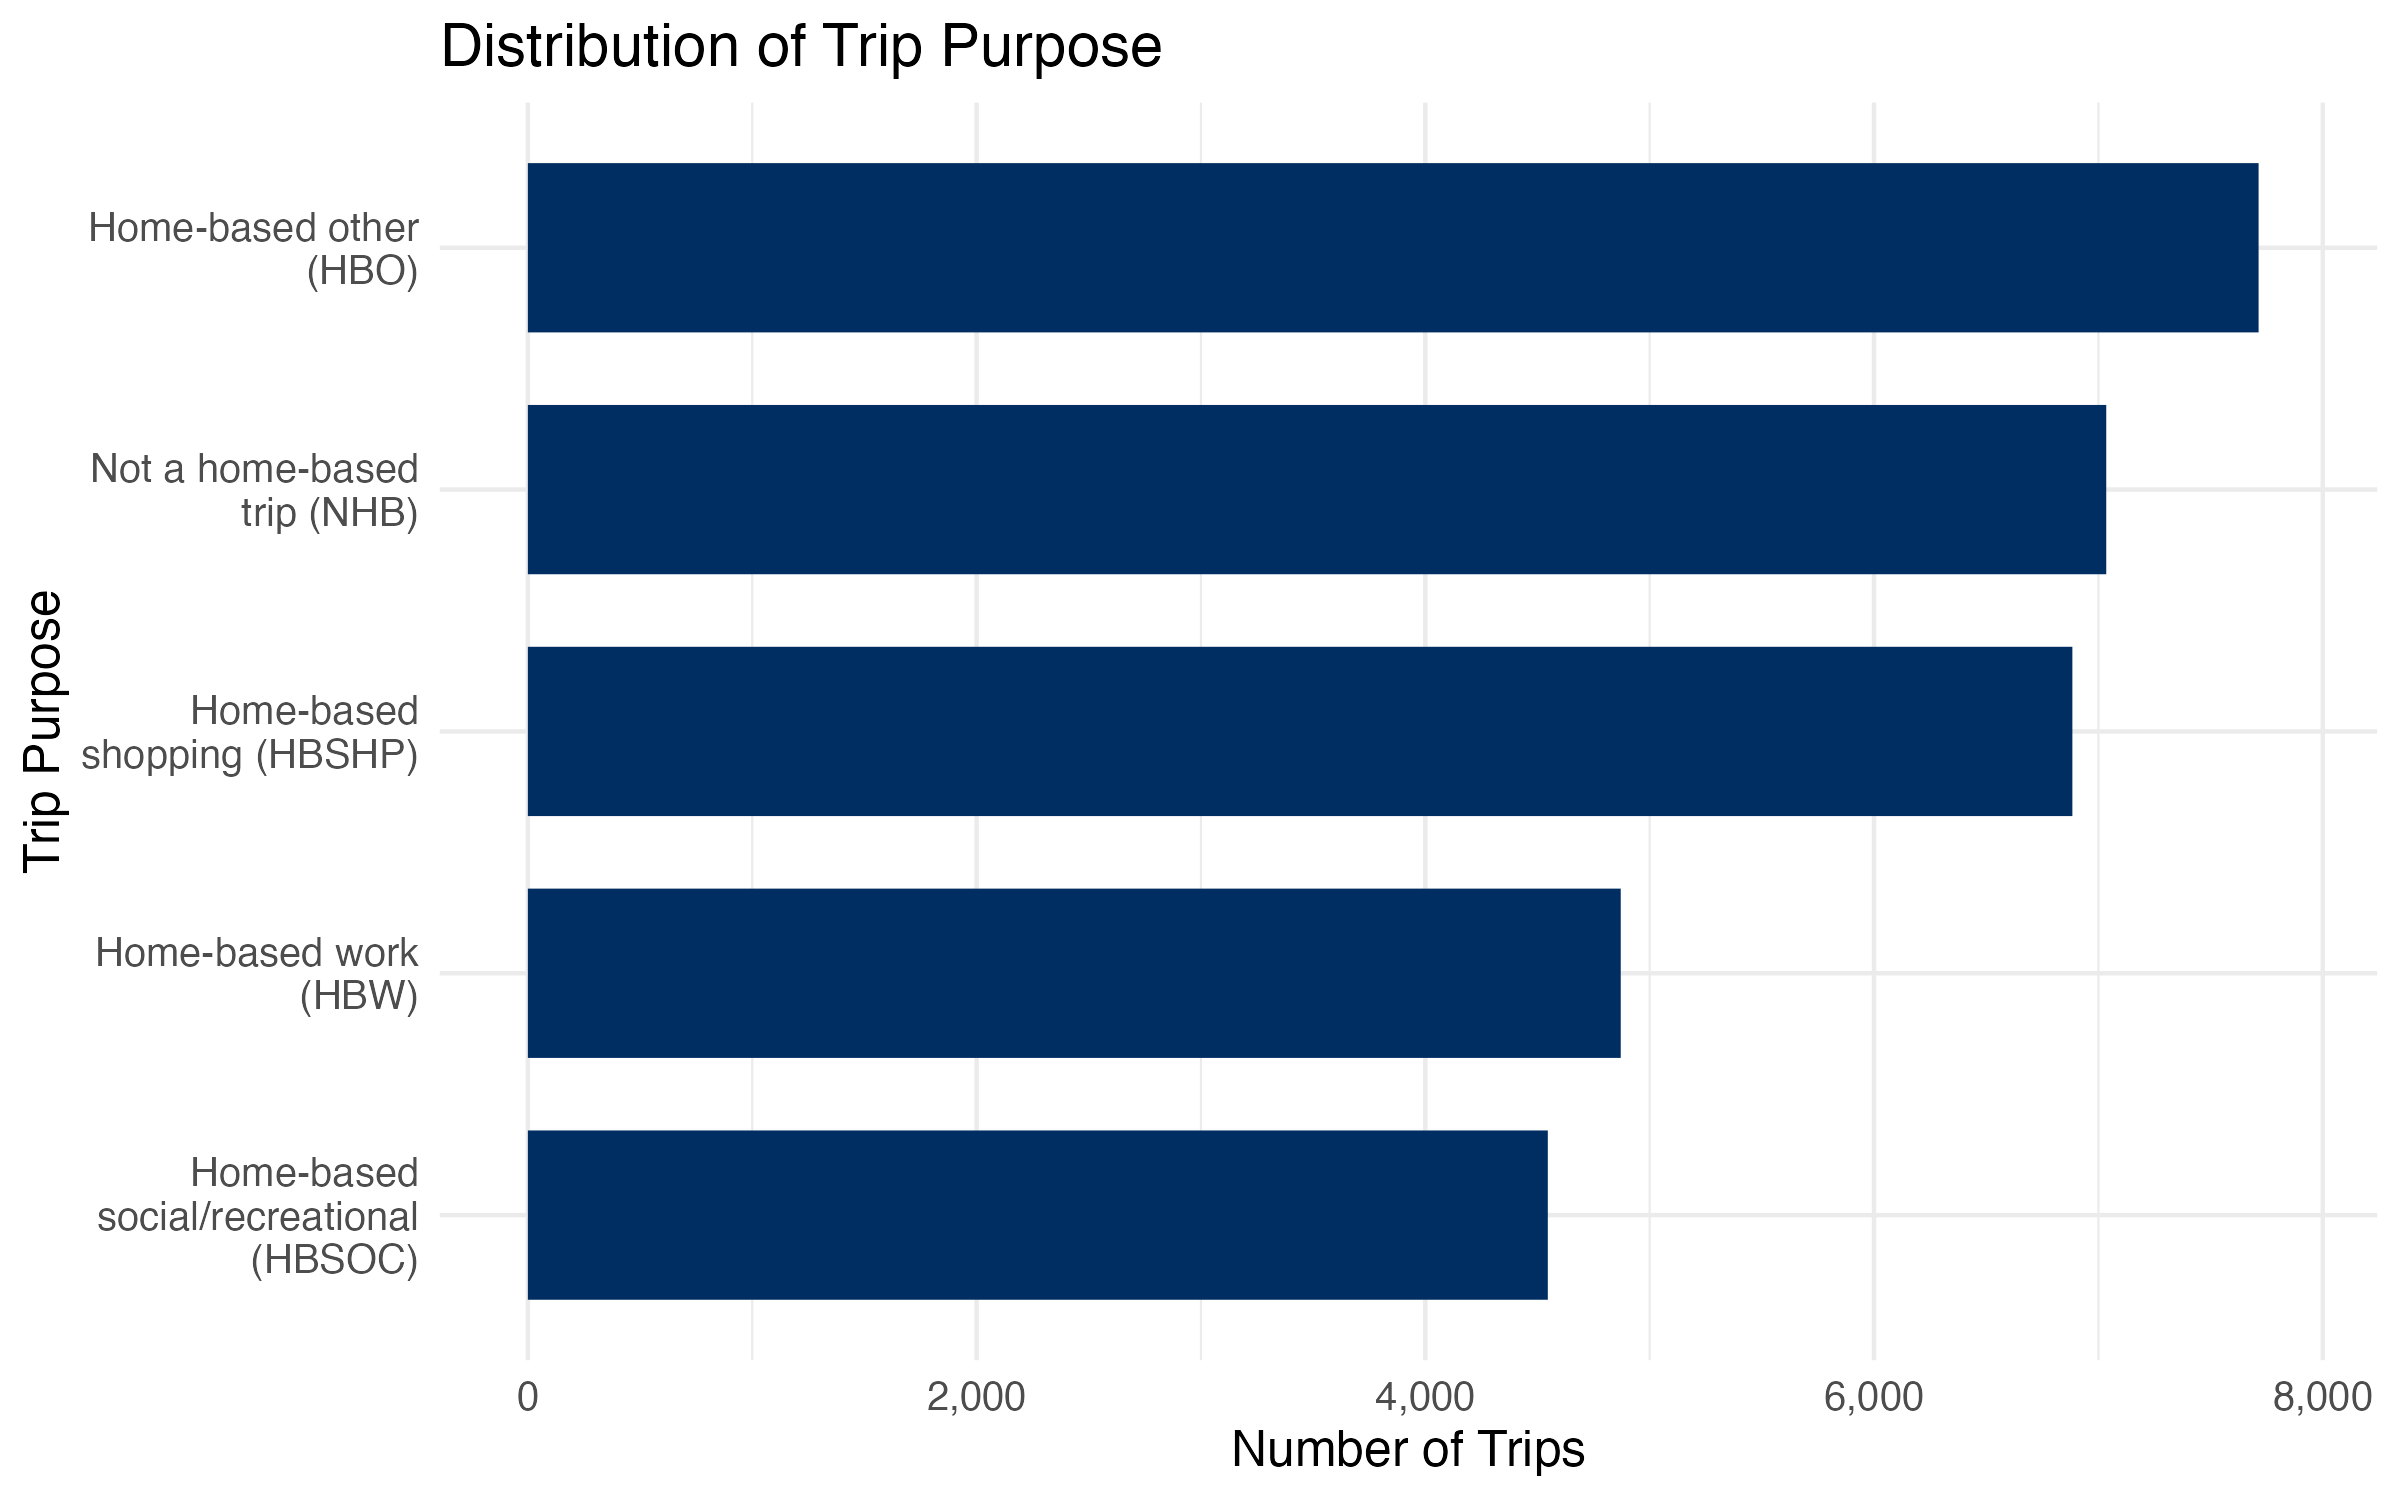
\includegraphics[width=0.7\textwidth,height=\textheight]{../code/poster/trip-purpose-distribution.png}

}

\caption{\label{fig-trip-purpose}Support of trip purpose, the target
variable for modeling.}

\end{figure}%

An analysis of the target variable support shows that the classes are
fairly balanced. While there is a distinction between the class sizes,
each class has a significantly large sample size to create a fairly
unbiased model. Modeling will be assess using balanced metrics in order
to verify that final results remain unbiased by class imbalance.

For all modeling, numerical predictors were scaled and centered to
normalize predictive influence. Categorical predictors were one-hot
encoded, generating binary nomial predictors for each class level. The
final cleaned data set of \texttt{person} and \texttt{trip} data
contained 31,050 observations, 71 predictors, and one target variable.

\subsection{Statistical Modeling}\label{statistical-modeling}

In order to predict trip purpose using NHTS data, we trained and
assessed five different statistical learning model architectures. We
aimed to establish a base line model and then test various methods in
order to improve the predictive power of the statistical learning. Our
goal was to achieve a high predictive accuracy and a high ROC AUC score,
creating a model with strong predictive power and balanced results.

All statistical models were trained with 80\% of the data, using k-fold
cross validation for hypertuning parameters. Models were hypertuned
using grid search techniques in order to find the most appropriate
hyperparameters. Final results were assessed on the remaining 20\% of
the data.

\subsubsection{Logistic Regression}\label{logistic-regression}

In order to establish a base line predictive model, we first trained a
logistic regression model on the training data set. The logistic model
was trained on 22,356 observations of the data. We utilized 5-fold cross
validation to hypertune the models. Hypertuning was utilized for
regularization penalty type, regularization penalty value, and optimizer
values. We utilized a one-vs-rest strategy to account for the multiclass
nature of our data, meaning that each iterations trained 5 versions of
the model comparing one target class level with all other classes.

\subsubsection{Support Vector Machine}\label{support-vector-machine}

Next, a support vector machine was trained on the training data set to
classify the data. The support vector classifier was hypertuned using
5-fold cross validation. The model was hypertuned for the \(L2^2\)
regularization penalty value and kernel type. All models were training
with a one-vs-rest strategy for the multiclass problem. The final model
was trained to generate probabilistic predictions using Scikit-learn's
\texttt{predict\_proba()} function and a pairwise coupling strategy.

\subsubsection{Neural Network}\label{neural-network}

We designed and trained a neural network to predict trip purposes using
\texttt{keras}. Extensive hypertuning using 5-fold cross validation
included tuning for the optimizer's learning rate, hidden unit size,
dropout regularization levels, and activation functions. The final model
was a linear deep feed forward multilayer perceptron with 2 hidden
layers. Both hidden layers have a hidden size of 64 and utilize
sigmoidal activation. After hypertuning, we found that the best model
used no regularization, so the dropout level was 0. The output layer
uses softmax to output predicted probabilities that the observation
belongs in each of the five target classes. The model was trained with a
patience level of two epochs and utilized 10\% of the training data as a
validation set to implement early stopping. The loss function was
categorical crossentropy and the optimizer was Adam.

\subsubsection{Random Forest}\label{random-forest}

A random forest classifier was utilized to predict trip purpose from the
observations. We trained a random forest classifier using 5-fold cross
validation to find the best hyperparameters. Hyperparameter search
included the maximum depth of branches, minimum number of samples
requires to split a leaf, and the number of trees (estimators) in the
forest. The best model was selected as the model with the highest
accuracy.

\subsubsection{XGBoost}\label{xgboost}

Finally, an XGBoost classifier was trained to predict trip purpose from
our training data. The XGBoost model was hypertuned for maximum tree
depth, learning rate of the optimizer, number of trees (estimators), the
minimum loss reduction required to split a leaf (also called gamma), the
subsampling ratio for preventing overfitting, and the subsample size of
the columns used by each tree. XGBoost was hypertuned using 3-fold cross
validation and a random grid search.

\section{Results}\label{results}

We observe that the XGBoost machine learning algorithm performed the
best with a test accuracy of 82.17\% followed by a Random Forest model
which had an accuracy of 73.22\%. A neural network model was also fit to
the data but it only resulted in an accuracy of 59.88\%, followed by
Support Vector Machines and Logistic Regression which had accuracy rates
of 51.21\% and 45.67\%.

\begin{center}
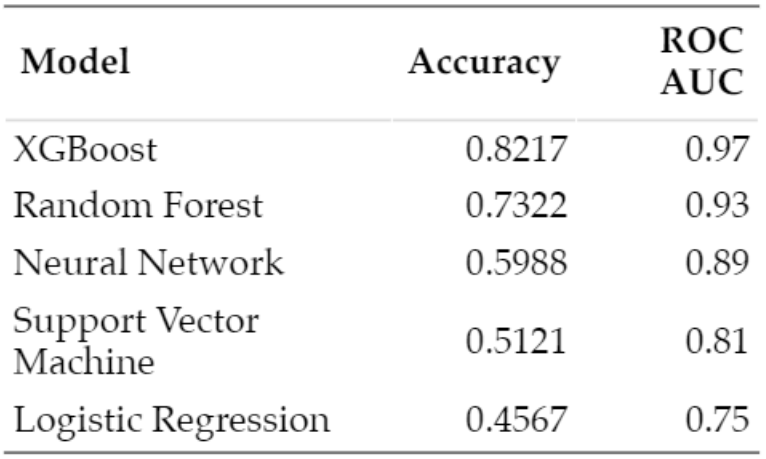
\includegraphics[width=0.6\textwidth,height=\textheight]{imgs/Screenshot.png}
\end{center}

We also observed the ROC AUC curve to be the greatest for XGBoost
model-0.97, followed by Random Forest which had the ROC AUC curve of
0.93. Overall, XGBoost model performed the best out of all the five
models that were trained on the data.

\begin{center}
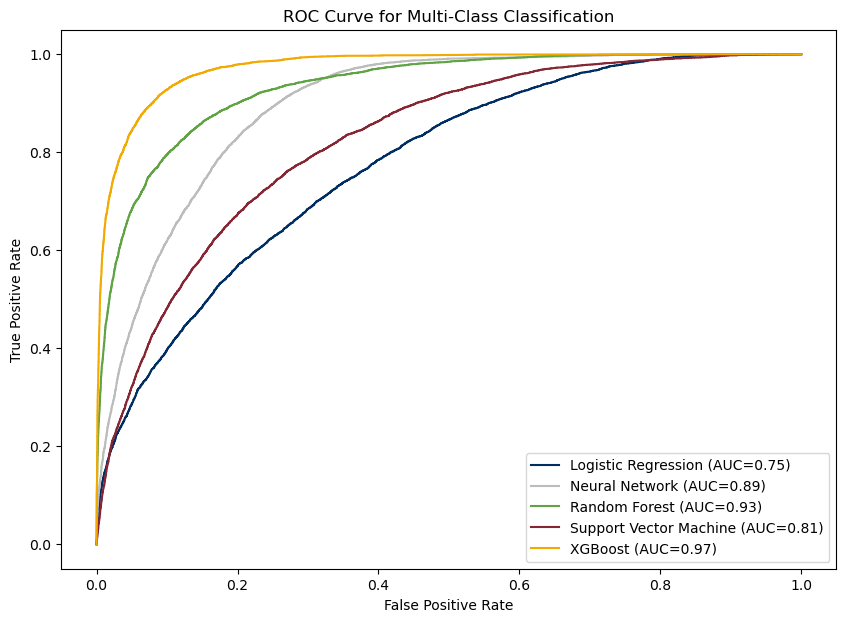
\includegraphics[width=0.75\textwidth,height=\textheight]{imgs/roc-auc.png}
\end{center}

We also observe the predicted probability for different classes for
different models that were trained. As observed, the mean predicted
probability for each class for the XGBoost model appears to be between
0.75 and 1.00 which displays the high likelihood that the data point
belongs to that particular class. Almost all other algorithms perform
much poorly compared to XGBoost

\begin{center}
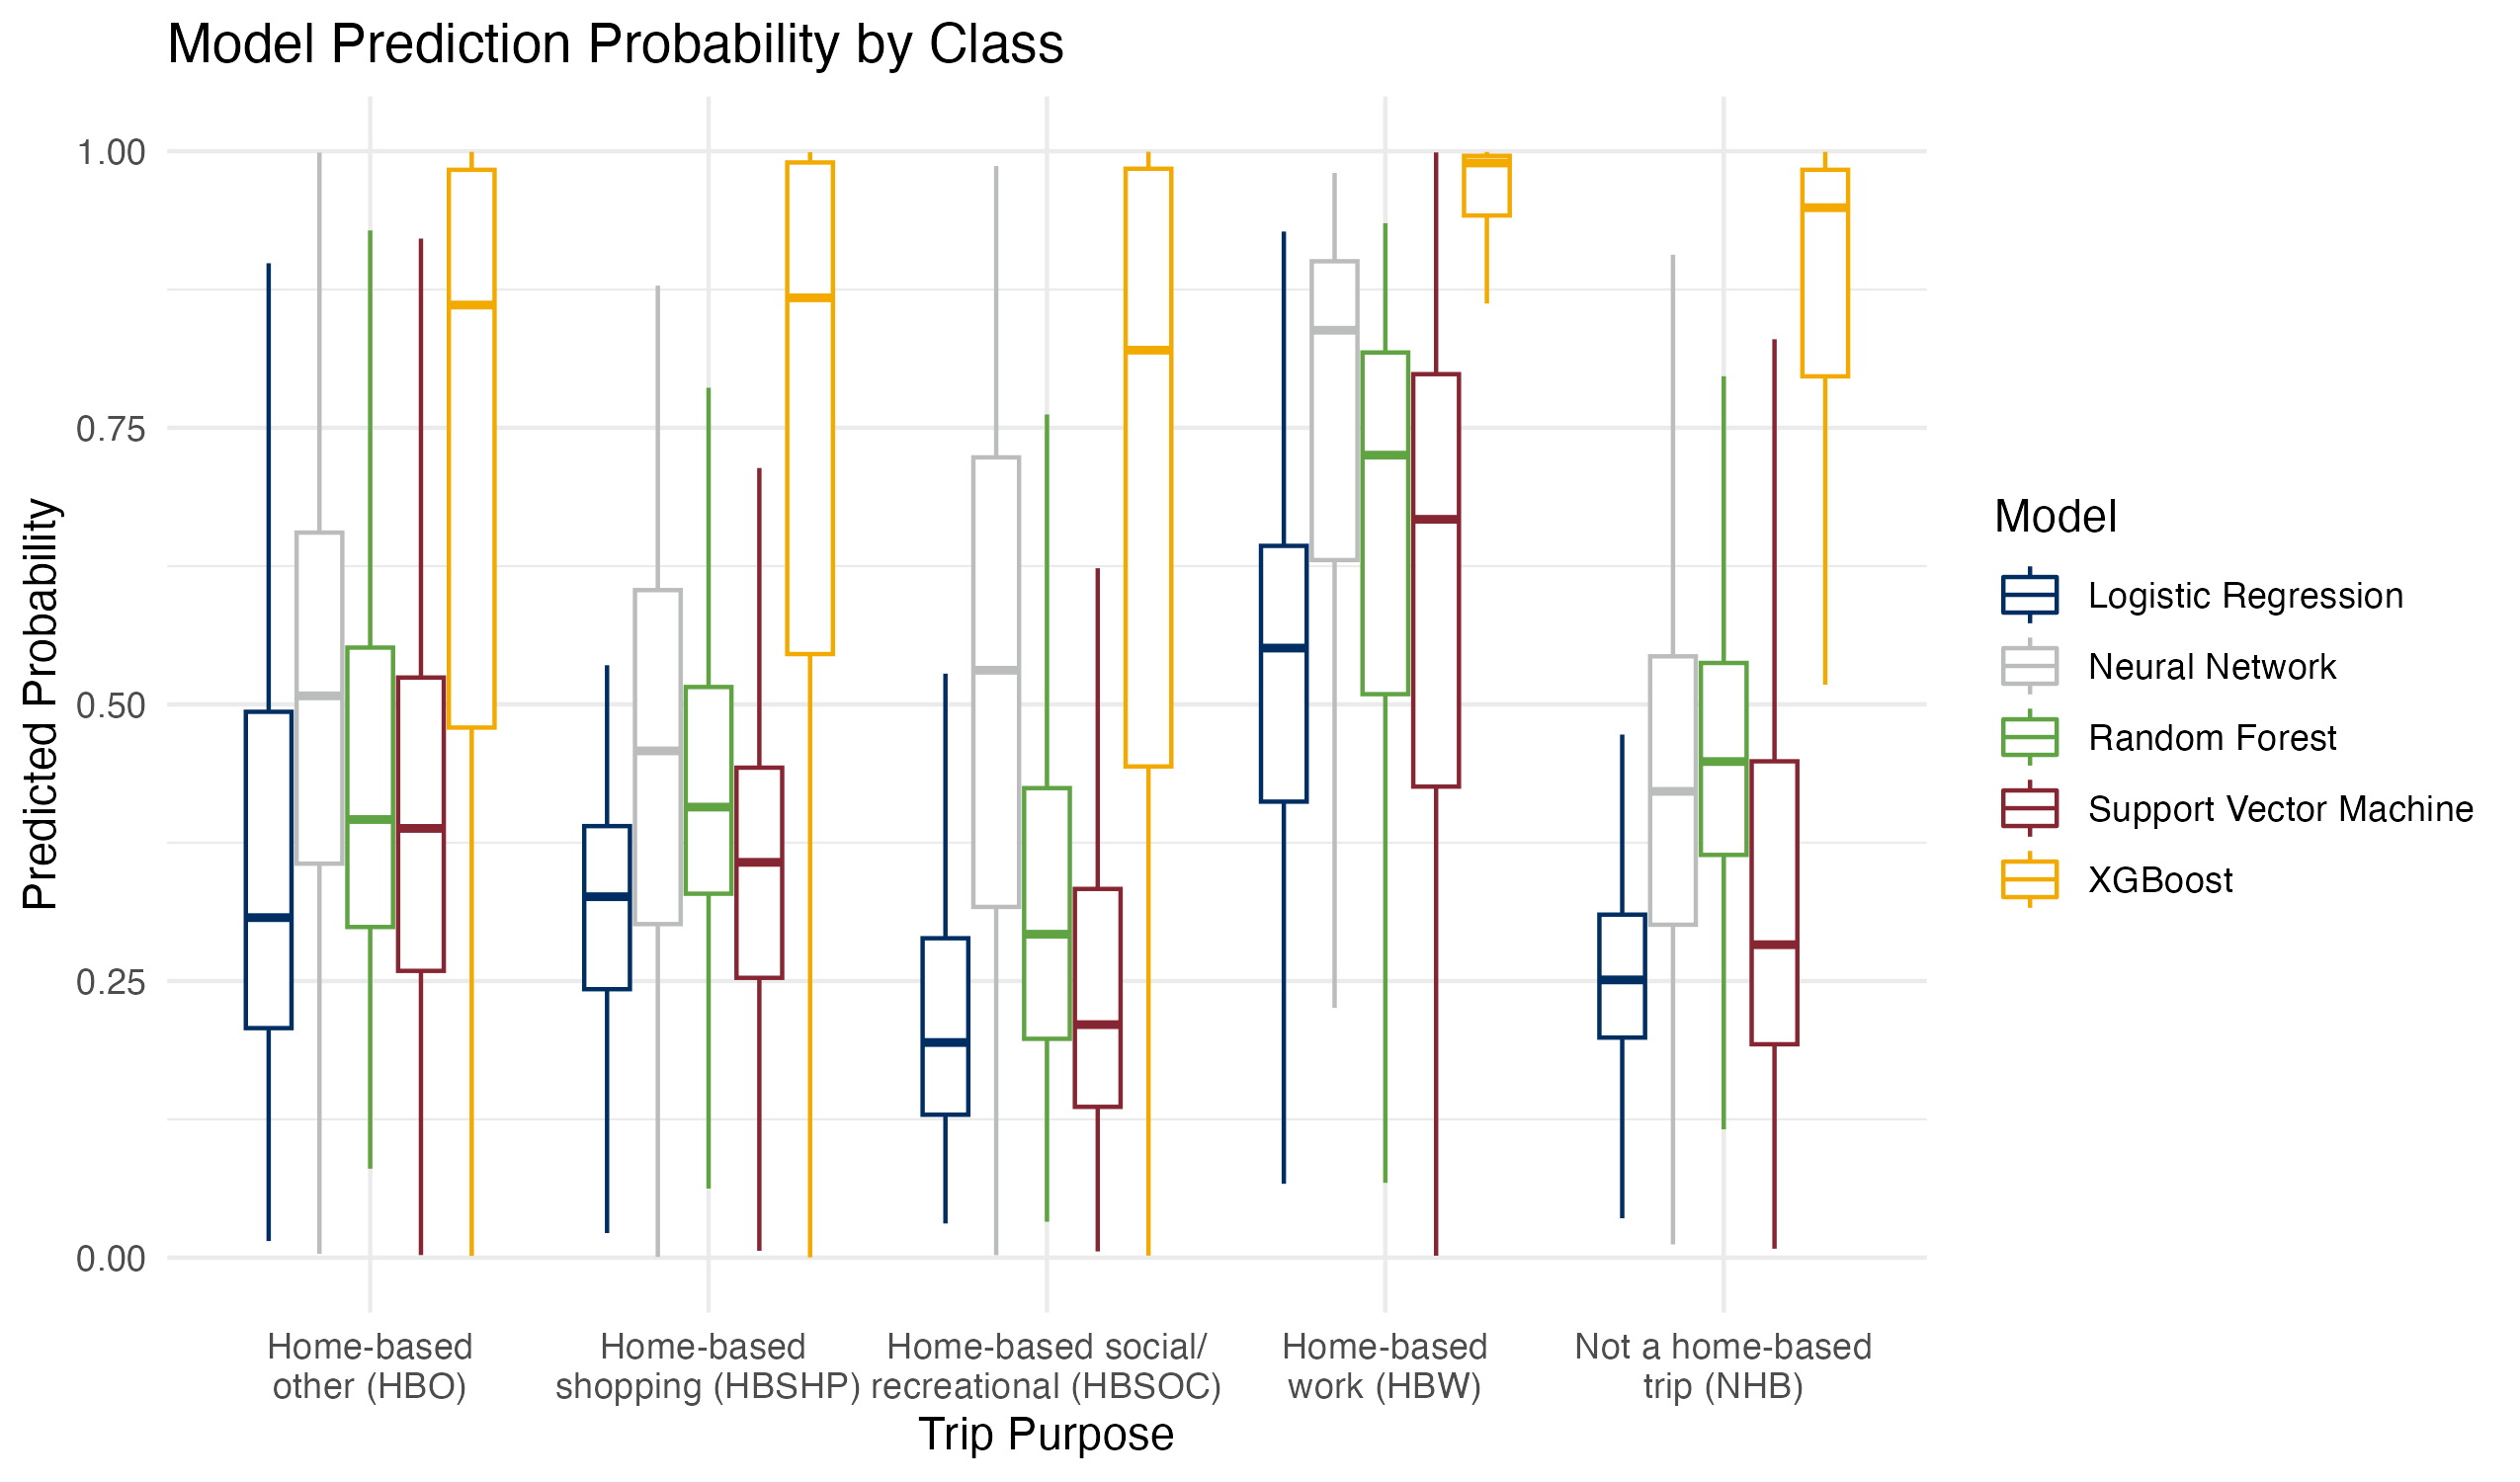
\includegraphics[width=0.75\textwidth,height=\textheight]{imgs/model-prediction-certainty-by-class.png}
\end{center}

\section{Discussion}\label{discussion}

Among all the models considered, XGBoost stands out as the best
performer, followed closely by Random Forest. Both XGBoost and Random
Forest are ensemble methods that have the ability to achieve low
variance and bias by leveraging weak estimators to build strong
classifiers. However, XGBoost exhibits certain advantages over Random
Forest. XGBoost incorporates a gradient boosting framework that enables
it to handle more complex relationships within the data. This allows
XGBoost to learn complex patterns and interactions within the data and
achieves a better predictive performance.

Neural networks also have the potential to capture complex patterns
within the data. However, they come with a trade-off in terms of their
computational intensity. Neural networks require significant
computational resources and time to train, especially when dealing with
large datasets or complex architectures.

SVM and logistic regression, while being widely used classification
algorithms, did not perform as well in this context. The complexity of
the underlying data seems to pose a challenge for these models. SVM
relies on finding optimal hyperplanes to separate data points, and
logistic regression assumes a linear relationship between the features
and the target variable. These assumptions may not hold true for the
given dataset based on the result.

One notable advantage of XGBoost and Random Forest is their
interpretability, or XAI (explainable artificial intelligence). These
models provide insights into feature importance, allowing us to
understand the factors driving the estimation of travel purposes. From
the analysis, it is evident that the ``reason\_for\_travel'' and
``time\_at\_destination'' features hold the most significant importance
in estimating the travel purpose. This aligns with our intuition as
these features likely contain patterns that strongly correlate with
determining the travel purpose. That being said, the features were
checked against trip\_purpose for multicollinearity and none was found.
It is important to note that while the feature names trip\_purpose and
reason\_for\_trip sound similar, they are measuring different things.
For example, ``Buy meals'' appears frequently in the reason\_for\_travel
feature, but it appears in home based shopping, social and recreational,
and not home based shopping. In contrast, interpreting neural network
models and SVMs can be challenging due to their more complex internal
workings and lack of feature importance measures.

\section{Conclusion}\label{conclusion}

Based on this study, we can see that tree-based methods, especially
XGBoost, have the best results for predicting trip purpose from NHTS
data in 2022. The most important features in this model include the
reason for travel, worker status, the trip destination, and whether the
trip occurred over the weekend. Our best test accuracy from the XGBoost
model was 82.17\%, which is nearly double the best test accuracy
achieved by the baseline logistic regression model. Our ability to
predict trip purpose with high accuracy and ROC AUC suggests that trip
purpose is explainable by trip characteristics and demographic
information.

There are many potential future applications that can be based on the
findings in this study. One possible future application would be to move
from using survey data to observed data. Similar data could be collected
by taxi or ride sharing companies like Uber or Lyft, and the predicted
trip purpose could be used to to better determine how many cars will be
needed in certain areas. Similar trip characteristics and demographic
information can be collected by many other types of businesses and
organizations from hotel chains to environmental researchers. Being able
to accurately predict the purposes of trips will have significant impact
for hotel chains by allowing them to predict where more capacity will be
needed and how specific hotels can be expected to perform. Similarly,
accurate trip purpose predictions will allow climate researchers to
determine where to target efforts for future green house gas emission
reductions. For example, places and trip modalities that are mostly used
for work are unlikely to be easily changed, while trip modalities that
are used mostly for recreation may be more easily targeted for
reductions.

Lastly, there are several ways in which the models examined in this
study may be enhanced in the future. Our full dataset contained over 60
different features to be used by our models. By applying a feature
selection or dimensionality reduction algorithm like PCA or t-SNE we
could remove the features with the lowest importance to our final
models. This may allow the models to perform better. One area of future
research would be to examine how adding past NHTS survey data effects
the predictions. This would give us a better idea of how reliable our
predictions may be in the future based on similar survey data.

\phantomsection\label{refs}
\begin{CSLReferences}{1}{0}
\bibitem[\citeproctext]{ref-fhwa2022nhts}
Federal Highway Administration. 2022a. {``{2022 NextGen National
Household Travel Survey Core Data}.''} Washington, DC: {U.S. Department
of Transportation}; Available online. \url{http://nhts.ornl.gov}.

\bibitem[\citeproctext]{ref-nhtsfaq}
---------. 2022b. {``{2022 NHTS Frequently Asked Questions}.''}
\emph{{National Household Travel Survey}}. {U.S. Department of
Transportation}; Available online; {Federal Highway Administration}.
\url{https://nhts.ornl.gov/faq}.

\bibitem[\citeproctext]{ref-Compendium}
---------. 2023. {``National Household Travel Survey Compendium of
Uses.''} Published by Federal Highway Administration {[}Online{]}.
\url{https://nhts.ornl.gov/assets/2023_compendium.pdf}.

\bibitem[\citeproctext]{ref-LU2023189}
Lu, Yougeng, and Genevieve Giuliano. 2023. {``Understanding Mobility
Change in Response to COVID-19: A Los Angeles Case Study.''}
\emph{Travel Behaviour and Society} 31: 189--201.
https://doi.org/\url{https://doi.org/10.1016/j.tbs.2022.11.011}.

\bibitem[\citeproctext]{ref-Paul2023}
Paul, Julene. 2023. {``Sharing in and Sharing Out: The Equity
Implications of Informal Vehicle-Sharing.''} UCLA.

\end{CSLReferences}



\end{document}
